% !TeX spellcheck = en_US
\documentclass[./main.tex]{subfiles}
\begin{document}
	 \subsection{Chat implementation}
	 In this subsection it shall be described how and why the Chat implementations was done as it
	 is today in the backend. The technologies that were used for providing the Chat was a simple 
	 WebSocket. They have been a standard since 2015 and have been widely adapted to browsers,
	 as well as in flutter, so it is an easy development on both web and mobile app. \\
	 \\
	 As for the server, this is done with an official Django library called \textit{django-channels}, but the requirements on the server change to be able to hold this application. The websockets are connected to a \textit{room chat}, that resents every message to all the others clients that are connected on this room.\\
	 \\
	 This happens asynchronously in the server, which makes the integration for this server so different from the other services, as the server runner has to be changed accordingly to be able to hold the  \textit{asgy} application.\footnote{Python has two standards for web servers, one called \textit{wsgi} for  synchronous servers, and the other called \textit{asgi}. Django was done with \textit{wsgi} in mind, but,  in recent years, development has been made so that it can use \textit{asgi}.}
	 \\
	 \\
	 Another problem that we had upon the application was that websockets don't have memory, so you can't ask for the messages from a chat in the websocket. At first, it was thought  that this would be managed by the library itself, as it uses Redis for escalating the websockets, but it was found out that it cannot achieve this use case. For this reason, the database model was changed to hold the messages from a chat.\\
	 \\
	 So, seen it as a sequence diagram, the chat has to be implemented following the next calls:
 \begin{figure}[H]
 	\centering
 	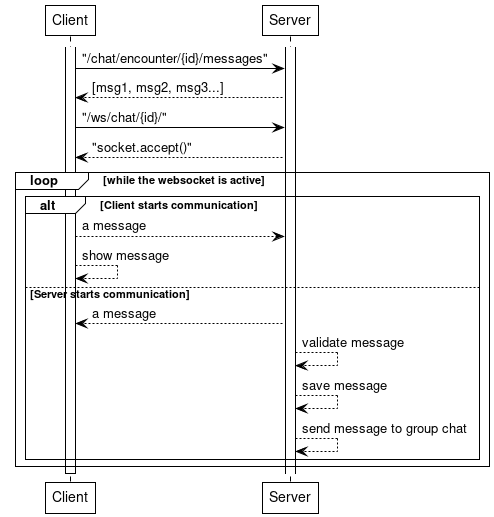
\includegraphics[width=0.6\textwidth]{img/api-calls.png}
 	\caption{General architecture of the application.}
 \end{figure}
	 
\end{document}